 \documentclass{article}
\usepackage[utf8]{inputenc}
\usepackage[a4paper, total={7in, 10in}]{geometry}
\usepackage{braket}
\usepackage{xcolor}
\usepackage{amsmath}
\usepackage{amssymb}
\usepackage{amsfonts}
\usepackage{graphicx}
\usepackage{svg}
\usepackage{float}
\usepackage{tikz}
\usepackage[ruled,vlined]{algorithm2e}
\usepackage{multicol}
\usepackage[backend=biber,style=alphabetic,sorting=ynt]{biblatex}
\usepackage{xcolor}
%\addbibresource{sample.bib} %Import the bibliography file

\newcommand{\commentt}[1]{\textcolor{blue}{ \textbf{[COMMENT]} #1}}
\newcommand{\ctt}[1]{\commentt{#1}}
\newcommand{\prb}[1]{ \mathbf{Pr} \left[ {#1} \right]}
\newcommand{\onotation}[1]{\(\mathcal{O} \left( {#1}  \right) \)}
\newcommand{\ona}[1]{\onotation{#1}}
\newcommand{\PSI}{{\ket{\psi}}}
\newcommand{\LESn}{\ket{\psi_n}}
\newcommand{\LESa}{\ket{\phi_n}}
\newcommand{\LESs}{\frac{1}{\sqrt{n}}\sum_{i}{\ket{\left(0^{i}10^{n-i}\right)^{n}}}}
\newcommand{\Hn}{\mathcal{H}_{n}}
\newcommand{\Ep}{\frac{1}{\sqrt{2^n}}\sum^{2^n}_{x}{ \ket{xx}}}
\newcommand{\HON}{\ket{\psi_{\text{honest}}}}
\newcommand{\Lemma}{\paragraph{Lemma.}}


\setlength{\columnsep}{0.6cm}

\newcommand{\Gz}{ G_{z}^{\delta} } 

\begin{document}

\title{Quantum LTC With Positive Rate}
\author{David Ponarovsky}
\maketitle
%\begin{multicols*}{2}
\newcommand{ \Hw }{ \delta\Delta -\Delta^{\frac{1}{2}-\varepsilon}/\delta  }
	\newcommand{ \Nw }{ \Delta^{\frac{3}{2}-\varepsilon}} 
	  \newcommand{ \Gu } { \Gamma^{\cup} }
	  \newcommand{ \Guq } { \Gamma^{\cup, \square} }

    	\newcommand{ \Gsa } {\Gamma_{\square_{1}} }
	\newcommand{ \Gsb } {\Gamma_{\square_{2}} }
        \newcommand{ \Aa } { C_{A_{1}}}  
	\newcommand{ \Ab } { C_{A_{2}}}
	\newcommand{ \Ac } { C_{A_{3}}}
	\newcommand{ \Aab } { \Aa \otimes \Ab } 
	\newcommand{ \Aac } { \Aa \otimes \Ac }
	\newcommand{ \Aabc } { \Aa \otimes \Ab \otimes \Ac }
	\newcommand{ \Aabp } { \Aa^{\perp} \otimes \Ab^{\perp} } 
	\newcommand{ \Aacp } { \Aa^{\perp} \otimes \Ac^{\perp} }
	\newcommand{ \Aabcp } { \Aa^{\perp} \otimes \Ab^{\perp} \otimes \Ac^{\perp} }
	\newcommand{ \Aabpp } { \left( \Aabp \right)^\perp } 
	\newcommand{ \Aacpp } { \left( \Aacp \right)^\perp }
	\newcommand{ \Aabcpp } { \left( \Aabcp \right)^\perp }
	\newcommand{ \YY } {  y_{1}y_{2}^{\top} }
	\newcommand{ \ZZ } {  z_{1}z_{2}^{\top} } 
	\newcommand{ \TT } { \tilde{\tau} } 


  \paragraph{preamble.} preamble.  
  \begin{figure}[H]
            %\label{fig:square}
            \begin{center}
            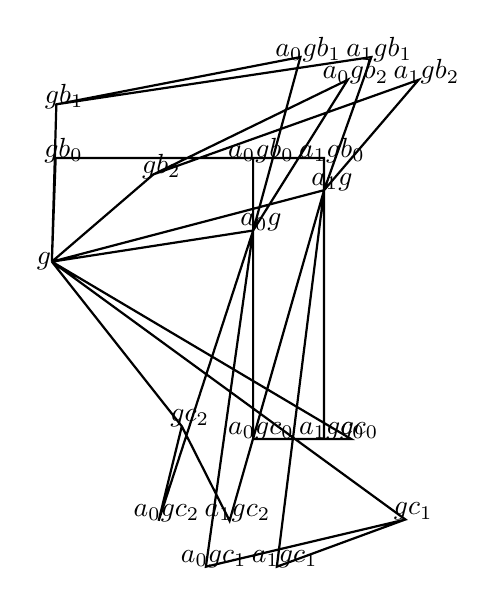
\begin{tikzpicture}
            \draw[thick](0,0)(0,0) -- (0.04822442375612579,1.3166731275257617) -- (2.556110328998928,1.3166731275257617) -- (2.556110328998928,0.39555356325843904) -- (0,0)
(0,0) -- (0.05695314073901281,1.9983534967390502) -- (3.156110328998928,2.5983534967390503) -- (2.556110328998928,0.39555356325843904) -- (0,0)
(0,0) -- (1.2905480160668374,1.1087835990202297) -- (3.756110328998928,2.30878359902023) -- (2.556110328998928,0.39555356325843904) -- (0,0)
(0,0) -- (0.04822442375612579,1.3166731275257617) -- (3.4569473286345382,1.3166731275257617) -- (3.4569473286345382,0.9079497284104932) -- (0,0)
(0,0) -- (0.05695314073901281,1.9983534967390502) -- (4.056947328634538,2.5983534967390503) -- (3.4569473286345382,0.9079497284104932) -- (0,0)
(0,0) -- (1.2905480160668374,1.1087835990202297) -- (4.656947328634538,2.30878359902023) -- (3.4569473286345382,0.9079497284104932) -- (0,0)
(0,0) -- (3.8013460418688565,-2.2526656347296123) -- (2.556110328998928,-2.2526656347296123) -- (2.556110328998928,0.39555356325843904) -- (0,0)
(0,0) -- (4.489718675054821,-3.2741071101675674) -- (1.956110328998928,-3.8741071101675675) -- (2.556110328998928,0.39555356325843904) -- (0,0)
(0,0) -- (1.6501944236515493,-2.09070808021107) -- (1.356110328998928,-3.29070808021107) -- (2.556110328998928,0.39555356325843904) -- (0,0)
(0,0) -- (3.8013460418688565,-2.2526656347296123) -- (3.4569473286345382,-2.2526656347296123) -- (3.4569473286345382,0.9079497284104932) -- (0,0)
(0,0) -- (4.489718675054821,-3.2741071101675674) -- (2.856947328634538,-3.8741071101675675) -- (3.4569473286345382,0.9079497284104932) -- (0,0)
(0,0) -- (1.6501944236515493,-2.09070808021107) -- (2.2569473286345385,-3.29070808021107) -- (3.4569473286345382,0.9079497284104932) -- (0,0)
;
\node at (2.656110328998928,1.4166731275257618) {$ a_{ 0  } gb_{ 0 } $};
\node at (3.256110328998928,2.6983534967390503) {$ a_{ 0  } gb_{ 1 } $};
\node at (3.8561103289989282,2.40878359902023) {$ a_{ 0  } gb_{ 2 } $};
\node at (3.5569473286345383,1.4166731275257618) {$ a_{ 1  } gb_{ 0 } $};
\node at (4.156947328634538,2.6983534967390503) {$ a_{ 1  } gb_{ 1 } $};
\node at (4.756947328634538,2.40878359902023) {$ a_{ 1  } gb_{ 2 } $};
\node at (2.656110328998928,-2.1526656347296123) {$ a_{ 0  } gc_{ 0 } $};
\node at (2.056110328998928,-3.7741071101675674) {$ a_{ 0  } gc_{ 1 } $};
\node at (1.4561103289989281,-3.19070808021107) {$ a_{ 0  } gc_{ 2 } $};
\node at (3.5569473286345383,-2.1526656347296123) {$ a_{ 1  } gc_{ 0 } $};
\node at (2.9569473286345382,-3.7741071101675674) {$ a_{ 1  } gc_{ 1 } $};
\node at (2.3569473286345386,-3.19070808021107) {$ a_{ 1  } gc_{ 2 } $};
\node at (-0.1,0) {$ g $};
\node at (2.656110328998928,0.495553563258439) {$ a_{ 0 }g $};
\node at (3.5569473286345383,1.0079497284104932) {$ a_{ 1 }g $};
\node at (0.1482244237561258,1.4166731275257618) {$ gb_{ 0 } $};
\node at (0.15695314073901281,2.0983534967390503) {$ gb_{ 1 } $};
\node at (1.3905480160668375,1.2087835990202298) {$ gb_{ 2 } $};
\node at (3.9013460418688566,-2.1526656347296123) {$ gc_{ 0 } $};
\node at (4.5897186750548205,-3.1741071101675673) {$ gc_{ 1 } $};
\node at (1.7501944236515494,-1.99070808021107) {$ gc_{ 2 } $};

            \end{tikzpicture}
            \end{center}
            \caption{Square of the complex, with edges $(g,ag), (agb, gb) \in E_A,
            (g,gb), (agb, ag) \in E_B.$ \label{fig:square}
            }
            \end{figure}
 \begin{figure}[H]
            %\label{fig:square}
            \begin{center}
            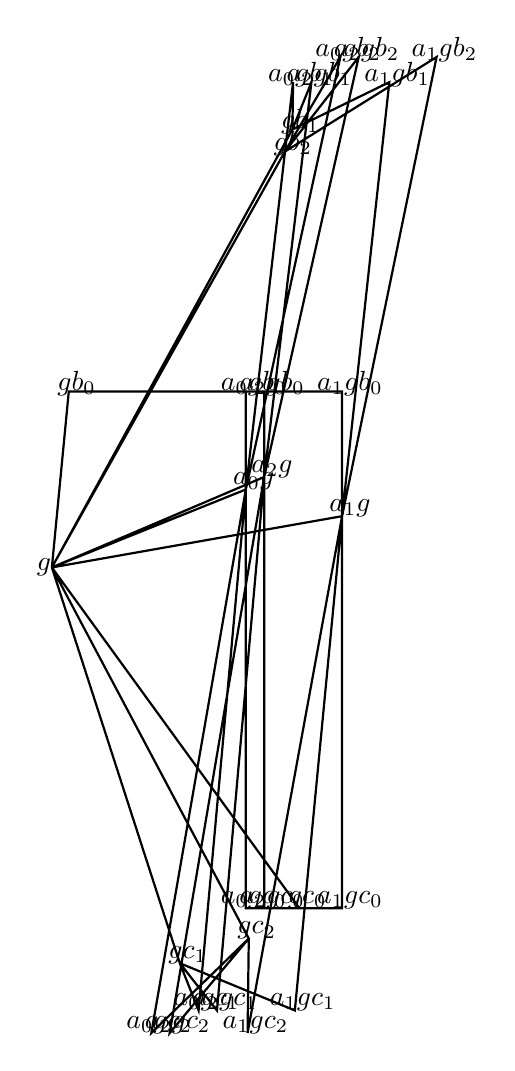
\begin{tikzpicture}
            \draw[thick](0,0)(0,0) -- (0.21474860383682848,2.2333099117351787) -- (2.4632440959746416,2.2333099117351787) -- (2.4632440959746416,0.9902456973064327) -- (0,0)
(0,0) -- (3.054722414367636,5.5625507292194145) -- (3.0632440959746416,6.162550729219414) -- (2.4632440959746416,0.9902456973064327) -- (0,0)
(0,0) -- (2.9597717102417915,5.281726095715909) -- (3.6632440959746413,6.481726095715909) -- (2.4632440959746416,0.9902456973064327) -- (0,0)
(0,0) -- (0.21474860383682848,2.2333099117351787) -- (3.685661096728061,2.2333099117351787) -- (3.685661096728061,0.6509588395094247) -- (0,0)
(0,0) -- (3.054722414367636,5.5625507292194145) -- (4.285661096728061,6.162550729219414) -- (3.685661096728061,0.6509588395094247) -- (0,0)
(0,0) -- (2.9597717102417915,5.281726095715909) -- (4.885661096728061,6.481726095715909) -- (3.685661096728061,0.6509588395094247) -- (0,0)
(0,0) -- (0.21474860383682848,2.2333099117351787) -- (2.6965740809653034,2.2333099117351787) -- (2.6965740809653034,1.14924313947216) -- (0,0)
(0,0) -- (3.054722414367636,5.5625507292194145) -- (3.2965740809653035,6.162550729219414) -- (2.6965740809653034,1.14924313947216) -- (0,0)
(0,0) -- (2.9597717102417915,5.281726095715909) -- (3.896574080965303,6.481726095715909) -- (2.6965740809653034,1.14924313947216) -- (0,0)
(0,0) -- (3.143816664620913,-4.328483051531332) -- (2.4632440959746416,-4.328483051531332) -- (2.4632440959746416,0.9902456973064327) -- (0,0)
(0,0) -- (1.6249218304328272,-5.026015355889664) -- (1.8632440959746415,-5.626015355889663) -- (2.4632440959746416,0.9902456973064327) -- (0,0)
(0,0) -- (2.5007390633138096,-4.712376246117253) -- (1.2632440959746416,-5.912376246117253) -- (2.4632440959746416,0.9902456973064327) -- (0,0)
(0,0) -- (3.143816664620913,-4.328483051531332) -- (3.685661096728061,-4.328483051531332) -- (3.685661096728061,0.6509588395094247) -- (0,0)
(0,0) -- (1.6249218304328272,-5.026015355889664) -- (3.085661096728061,-5.626015355889663) -- (3.685661096728061,0.6509588395094247) -- (0,0)
(0,0) -- (2.5007390633138096,-4.712376246117253) -- (2.4856610967280615,-5.912376246117253) -- (3.685661096728061,0.6509588395094247) -- (0,0)
(0,0) -- (3.143816664620913,-4.328483051531332) -- (2.6965740809653034,-4.328483051531332) -- (2.6965740809653034,1.14924313947216) -- (0,0)
(0,0) -- (1.6249218304328272,-5.026015355889664) -- (2.0965740809653033,-5.626015355889663) -- (2.6965740809653034,1.14924313947216) -- (0,0)
(0,0) -- (2.5007390633138096,-4.712376246117253) -- (1.4965740809653034,-5.912376246117253) -- (2.6965740809653034,1.14924313947216) -- (0,0)
;
\node at (2.5632440959746416,2.3333099117351788) {$ a_{ 0  } gb_{ 0 } $};
\node at (3.1632440959746417,6.262550729219414) {$ a_{ 0  } gb_{ 1 } $};
\node at (3.7632440959746414,6.581726095715909) {$ a_{ 0  } gb_{ 2 } $};
\node at (3.7856610967280613,2.3333099117351788) {$ a_{ 1  } gb_{ 0 } $};
\node at (4.385661096728061,6.262550729219414) {$ a_{ 1  } gb_{ 1 } $};
\node at (4.985661096728061,6.581726095715909) {$ a_{ 1  } gb_{ 2 } $};
\node at (2.7965740809653035,2.3333099117351788) {$ a_{ 2  } gb_{ 0 } $};
\node at (3.3965740809653036,6.262550729219414) {$ a_{ 2  } gb_{ 1 } $};
\node at (3.996574080965303,6.581726095715909) {$ a_{ 2  } gb_{ 2 } $};
\node at (2.5632440959746416,-4.228483051531333) {$ a_{ 0  } gc_{ 0 } $};
\node at (1.9632440959746416,-5.526015355889664) {$ a_{ 0  } gc_{ 1 } $};
\node at (1.3632440959746417,-5.812376246117253) {$ a_{ 0  } gc_{ 2 } $};
\node at (3.7856610967280613,-4.228483051531333) {$ a_{ 1  } gc_{ 0 } $};
\node at (3.185661096728061,-5.526015355889664) {$ a_{ 1  } gc_{ 1 } $};
\node at (2.5856610967280615,-5.812376246117253) {$ a_{ 1  } gc_{ 2 } $};
\node at (2.7965740809653035,-4.228483051531333) {$ a_{ 2  } gc_{ 0 } $};
\node at (2.1965740809653034,-5.526015355889664) {$ a_{ 2  } gc_{ 1 } $};
\node at (1.5965740809653035,-5.812376246117253) {$ a_{ 2  } gc_{ 2 } $};
\node at (-0.1,0) {$ g $};
\node at (2.5632440959746416,1.0902456973064327) {$ a_{ 0 }g $};
\node at (3.7856610967280613,0.7509588395094247) {$ a_{ 1 }g $};
\node at (2.7965740809653035,1.2492431394721601) {$ a_{ 2 }g $};
\node at (0.31474860383682846,2.3333099117351788) {$ gb_{ 0 } $};
\node at (3.1547224143676362,5.662550729219414) {$ gb_{ 1 } $};
\node at (3.0597717102417916,5.3817260957159085) {$ gb_{ 2 } $};
\node at (3.2438166646209132,-4.228483051531333) {$ gc_{ 0 } $};
\node at (1.7249218304328273,-4.926015355889664) {$ gc_{ 1 } $};
\node at (2.6007390633138097,-4.612376246117253) {$ gc_{ 2 } $};

            \end{tikzpicture}
            \end{center}
            \caption{Square of the complex, with edges $(g,ag), (agb, gb) \in E_A,
            (g,gb), (agb, ag) \in E_B.$ \label{fig:square}
            }
            \end{figure}
 \begin{figure}[H]
            %\label{fig:square}
            \begin{center}
            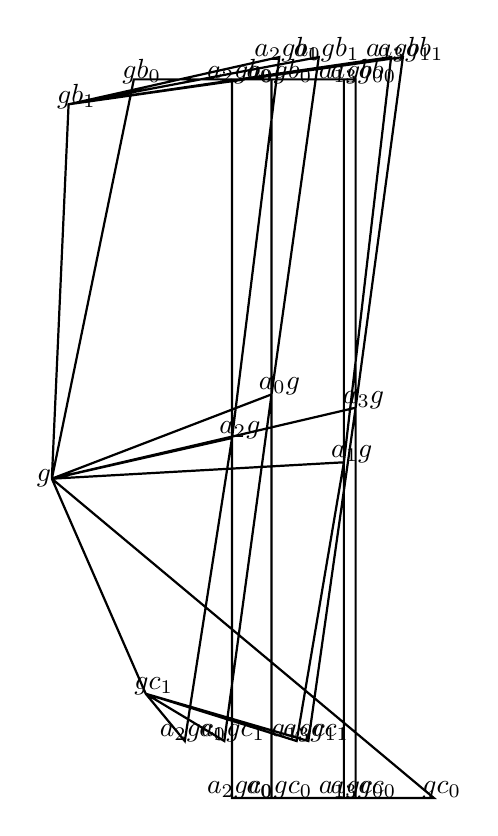
\begin{tikzpicture}
            \draw[thick](0,0)(0,0) -- (1.0411275354945597,5.07125501144667) -- (2.789793574987323,5.07125501144667) -- (2.789793574987323,1.0705261908881853) -- (0,0)
(0,0) -- (0.21230293845127257,4.7545516374206915) -- (3.389793574987323,5.354551637420691) -- (2.789793574987323,1.0705261908881853) -- (0,0)
(0,0) -- (1.0411275354945597,5.07125501144667) -- (3.708516445401308,5.07125501144667) -- (3.708516445401308,0.20813001746812645) -- (0,0)
(0,0) -- (0.21230293845127257,4.7545516374206915) -- (4.308516445401308,5.354551637420691) -- (3.708516445401308,0.20813001746812645) -- (0,0)
(0,0) -- (1.0411275354945597,5.07125501144667) -- (2.2878782399462425,5.07125501144667) -- (2.2878782399462425,0.516355349621797) -- (0,0)
(0,0) -- (0.21230293845127257,4.7545516374206915) -- (2.8878782399462426,5.354551637420691) -- (2.2878782399462425,0.516355349621797) -- (0,0)
(0,0) -- (1.0411275354945597,5.07125501144667) -- (3.857627267874706,5.07125501144667) -- (3.857627267874706,0.9014511591049392) -- (0,0)
(0,0) -- (0.21230293845127257,4.7545516374206915) -- (4.457627267874706,5.354551637420691) -- (3.857627267874706,0.9014511591049392) -- (0,0)
(0,0) -- (4.851481357026056,-4.055175791554876) -- (2.789793574987323,-4.055175791554876) -- (2.789793574987323,1.0705261908881853) -- (0,0)
(0,0) -- (1.1924473891194691,-2.731627456513865) -- (2.189793574987323,-3.331627456513865) -- (2.789793574987323,1.0705261908881853) -- (0,0)
(0,0) -- (4.851481357026056,-4.055175791554876) -- (3.708516445401308,-4.055175791554876) -- (3.708516445401308,0.20813001746812645) -- (0,0)
(0,0) -- (1.1924473891194691,-2.731627456513865) -- (3.108516445401308,-3.331627456513865) -- (3.708516445401308,0.20813001746812645) -- (0,0)
(0,0) -- (4.851481357026056,-4.055175791554876) -- (2.2878782399462425,-4.055175791554876) -- (2.2878782399462425,0.516355349621797) -- (0,0)
(0,0) -- (1.1924473891194691,-2.731627456513865) -- (1.6878782399462424,-3.331627456513865) -- (2.2878782399462425,0.516355349621797) -- (0,0)
(0,0) -- (4.851481357026056,-4.055175791554876) -- (3.857627267874706,-4.055175791554876) -- (3.857627267874706,0.9014511591049392) -- (0,0)
(0,0) -- (1.1924473891194691,-2.731627456513865) -- (3.257627267874706,-3.331627456513865) -- (3.857627267874706,0.9014511591049392) -- (0,0)
;
\node at (2.889793574987323,5.17125501144667) {$ a_{ 0  } gb_{ 0 } $};
\node at (3.4897935749873232,5.454551637420691) {$ a_{ 0  } gb_{ 1 } $};
\node at (3.8085164454013083,5.17125501144667) {$ a_{ 1  } gb_{ 0 } $};
\node at (4.4085164454013075,5.454551637420691) {$ a_{ 1  } gb_{ 1 } $};
\node at (2.3878782399462426,5.17125501144667) {$ a_{ 2  } gb_{ 0 } $};
\node at (2.9878782399462427,5.454551637420691) {$ a_{ 2  } gb_{ 1 } $};
\node at (3.957627267874706,5.17125501144667) {$ a_{ 3  } gb_{ 0 } $};
\node at (4.557627267874706,5.454551637420691) {$ a_{ 3  } gb_{ 1 } $};
\node at (2.889793574987323,-3.955175791554876) {$ a_{ 0  } gc_{ 0 } $};
\node at (2.289793574987323,-3.231627456513865) {$ a_{ 0  } gc_{ 1 } $};
\node at (3.8085164454013083,-3.955175791554876) {$ a_{ 1  } gc_{ 0 } $};
\node at (3.208516445401308,-3.231627456513865) {$ a_{ 1  } gc_{ 1 } $};
\node at (2.3878782399462426,-3.955175791554876) {$ a_{ 2  } gc_{ 0 } $};
\node at (1.7878782399462425,-3.231627456513865) {$ a_{ 2  } gc_{ 1 } $};
\node at (3.957627267874706,-3.955175791554876) {$ a_{ 3  } gc_{ 0 } $};
\node at (3.357627267874706,-3.231627456513865) {$ a_{ 3  } gc_{ 1 } $};
\node at (-0.1,0) {$ g $};
\node at (2.889793574987323,1.1705261908881854) {$ a_{ 0 }g $};
\node at (3.8085164454013083,0.30813001746812646) {$ a_{ 1 }g $};
\node at (2.3878782399462426,0.6163553496217969) {$ a_{ 2 }g $};
\node at (3.957627267874706,1.0014511591049393) {$ a_{ 3 }g $};
\node at (1.1411275354945598,5.17125501144667) {$ gb_{ 0 } $};
\node at (0.31230293845127255,4.854551637420691) {$ gb_{ 1 } $};
\node at (4.951481357026056,-3.955175791554876) {$ gc_{ 0 } $};
\node at (1.2924473891194692,-2.631627456513865) {$ gc_{ 1 } $};

            \end{tikzpicture}
            \end{center}
            \caption{Square of the complex, with edges $(g,ag), (agb, gb) \in E_A,
            (g,gb), (agb, ag) \in E_B.$ \label{fig:square}
            }
            \end{figure}
 \begin{figure}[H]
            %\label{fig:square}
            \begin{center}
            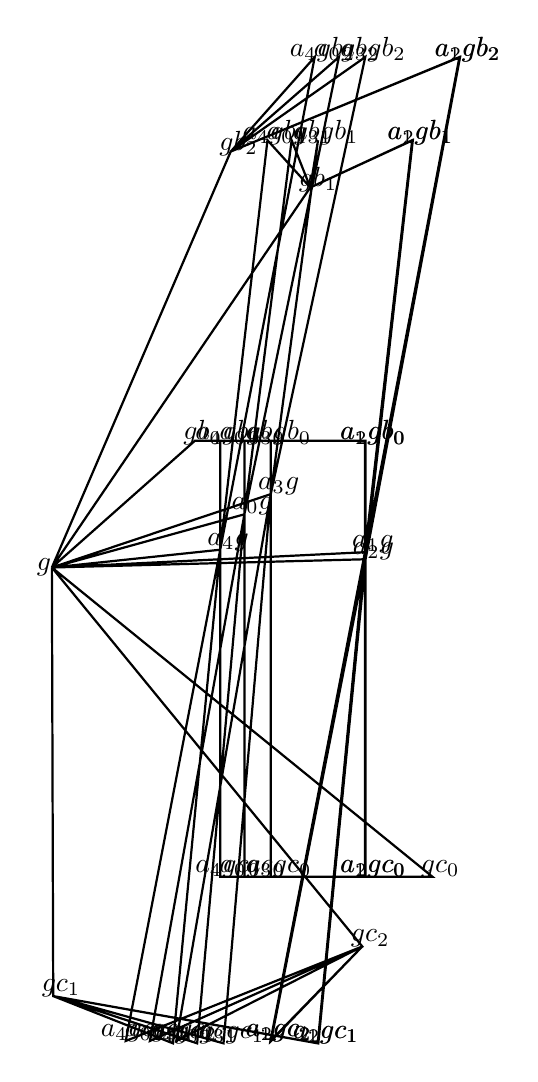
\begin{tikzpicture}
            \draw[thick](0,0)(0,0) -- (1.8152301038854846,1.6085116943634317) -- (2.4450541238798316,1.6085116943634317) -- (2.4450541238798316,0.675406741281627) -- (0,0)
(0,0) -- (3.2820212480038506,4.826150017168617) -- (3.0450541238798317,5.426150017168617) -- (2.4450541238798316,0.675406741281627) -- (0,0)
(0,0) -- (2.2713014465625996,5.282422077892296) -- (3.6450541238798317,6.482422077892296) -- (2.4450541238798316,0.675406741281627) -- (0,0)
(0,0) -- (1.8152301038854846,1.6085116943634317) -- (3.9761771475342798,1.6085116943634317) -- (3.9761771475342798,0.19444714330886817) -- (0,0)
(0,0) -- (3.2820212480038506,4.826150017168617) -- (4.576177147534279,5.426150017168617) -- (3.9761771475342798,0.19444714330886817) -- (0,0)
(0,0) -- (2.2713014465625996,5.282422077892296) -- (5.17617714753428,6.482422077892296) -- (3.9761771475342798,0.19444714330886817) -- (0,0)
(0,0) -- (1.8152301038854846,1.6085116943634317) -- (3.9840709357672726,1.6085116943634317) -- (3.9840709357672726,0.10474239951125881) -- (0,0)
(0,0) -- (3.2820212480038506,4.826150017168617) -- (4.584070935767272,5.426150017168617) -- (3.9840709357672726,0.10474239951125881) -- (0,0)
(0,0) -- (2.2713014465625996,5.282422077892296) -- (5.184070935767273,6.482422077892296) -- (3.9840709357672726,0.10474239951125881) -- (0,0)
(0,0) -- (1.8152301038854846,1.6085116943634317) -- (2.7797966648094716,1.6085116943634317) -- (2.7797966648094716,0.9323132989107913) -- (0,0)
(0,0) -- (3.2820212480038506,4.826150017168617) -- (3.3797966648094717,5.426150017168617) -- (2.7797966648094716,0.9323132989107913) -- (0,0)
(0,0) -- (2.2713014465625996,5.282422077892296) -- (3.979796664809472,6.482422077892296) -- (2.7797966648094716,0.9323132989107913) -- (0,0)
(0,0) -- (1.8152301038854846,1.6085116943634317) -- (2.138117140281164,1.6085116943634317) -- (2.138117140281164,0.22565735423080818) -- (0,0)
(0,0) -- (3.2820212480038506,4.826150017168617) -- (2.738117140281164,5.426150017168617) -- (2.138117140281164,0.22565735423080818) -- (0,0)
(0,0) -- (2.2713014465625996,5.282422077892296) -- (3.338117140281164,6.482422077892296) -- (2.138117140281164,0.22565735423080818) -- (0,0)
(0,0) -- (4.832608622126396,-3.9269830645971333) -- (2.4450541238798316,-3.9269830645971333) -- (2.4450541238798316,0.675406741281627) -- (0,0)
(0,0) -- (0.01710449904113731,-5.443072550697067) -- (1.8450541238798315,-6.043072550697067) -- (2.4450541238798316,0.675406741281627) -- (0,0)
(0,0) -- (3.942181799809523,-4.812865189017726) -- (1.2450541238798316,-6.0128651890177265) -- (2.4450541238798316,0.675406741281627) -- (0,0)
(0,0) -- (4.832608622126396,-3.9269830645971333) -- (3.9761771475342798,-3.9269830645971333) -- (3.9761771475342798,0.19444714330886817) -- (0,0)
(0,0) -- (0.01710449904113731,-5.443072550697067) -- (3.3761771475342797,-6.043072550697067) -- (3.9761771475342798,0.19444714330886817) -- (0,0)
(0,0) -- (3.942181799809523,-4.812865189017726) -- (2.7761771475342796,-6.0128651890177265) -- (3.9761771475342798,0.19444714330886817) -- (0,0)
(0,0) -- (4.832608622126396,-3.9269830645971333) -- (3.9840709357672726,-3.9269830645971333) -- (3.9840709357672726,0.10474239951125881) -- (0,0)
(0,0) -- (0.01710449904113731,-5.443072550697067) -- (3.3840709357672725,-6.043072550697067) -- (3.9840709357672726,0.10474239951125881) -- (0,0)
(0,0) -- (3.942181799809523,-4.812865189017726) -- (2.7840709357672724,-6.0128651890177265) -- (3.9840709357672726,0.10474239951125881) -- (0,0)
(0,0) -- (4.832608622126396,-3.9269830645971333) -- (2.7797966648094716,-3.9269830645971333) -- (2.7797966648094716,0.9323132989107913) -- (0,0)
(0,0) -- (0.01710449904113731,-5.443072550697067) -- (2.1797966648094715,-6.043072550697067) -- (2.7797966648094716,0.9323132989107913) -- (0,0)
(0,0) -- (3.942181799809523,-4.812865189017726) -- (1.5797966648094717,-6.0128651890177265) -- (2.7797966648094716,0.9323132989107913) -- (0,0)
(0,0) -- (4.832608622126396,-3.9269830645971333) -- (2.138117140281164,-3.9269830645971333) -- (2.138117140281164,0.22565735423080818) -- (0,0)
(0,0) -- (0.01710449904113731,-5.443072550697067) -- (1.5381171402811638,-6.043072550697067) -- (2.138117140281164,0.22565735423080818) -- (0,0)
(0,0) -- (3.942181799809523,-4.812865189017726) -- (0.9381171402811639,-6.0128651890177265) -- (2.138117140281164,0.22565735423080818) -- (0,0)
;
\node at (2.5450541238798317,1.7085116943634318) {$ a_{ 0  } gb_{ 0 } $};
\node at (3.1450541238798317,5.526150017168616) {$ a_{ 0  } gb_{ 1 } $};
\node at (3.745054123879832,6.5824220778922955) {$ a_{ 0  } gb_{ 2 } $};
\node at (4.076177147534279,1.7085116943634318) {$ a_{ 1  } gb_{ 0 } $};
\node at (4.676177147534279,5.526150017168616) {$ a_{ 1  } gb_{ 1 } $};
\node at (5.27617714753428,6.5824220778922955) {$ a_{ 1  } gb_{ 2 } $};
\node at (4.084070935767272,1.7085116943634318) {$ a_{ 2  } gb_{ 0 } $};
\node at (4.684070935767272,5.526150017168616) {$ a_{ 2  } gb_{ 1 } $};
\node at (5.284070935767272,6.5824220778922955) {$ a_{ 2  } gb_{ 2 } $};
\node at (2.8797966648094717,1.7085116943634318) {$ a_{ 3  } gb_{ 0 } $};
\node at (3.479796664809472,5.526150017168616) {$ a_{ 3  } gb_{ 1 } $};
\node at (4.0797966648094715,6.5824220778922955) {$ a_{ 3  } gb_{ 2 } $};
\node at (2.238117140281164,1.7085116943634318) {$ a_{ 4  } gb_{ 0 } $};
\node at (2.838117140281164,5.526150017168616) {$ a_{ 4  } gb_{ 1 } $};
\node at (3.438117140281164,6.5824220778922955) {$ a_{ 4  } gb_{ 2 } $};
\node at (2.5450541238798317,-3.826983064597133) {$ a_{ 0  } gc_{ 0 } $};
\node at (1.9450541238798316,-5.943072550697067) {$ a_{ 0  } gc_{ 1 } $};
\node at (1.3450541238798317,-5.912865189017727) {$ a_{ 0  } gc_{ 2 } $};
\node at (4.076177147534279,-3.826983064597133) {$ a_{ 1  } gc_{ 0 } $};
\node at (3.4761771475342798,-5.943072550697067) {$ a_{ 1  } gc_{ 1 } $};
\node at (2.8761771475342797,-5.912865189017727) {$ a_{ 1  } gc_{ 2 } $};
\node at (4.084070935767272,-3.826983064597133) {$ a_{ 2  } gc_{ 0 } $};
\node at (3.4840709357672726,-5.943072550697067) {$ a_{ 2  } gc_{ 1 } $};
\node at (2.8840709357672725,-5.912865189017727) {$ a_{ 2  } gc_{ 2 } $};
\node at (2.8797966648094717,-3.826983064597133) {$ a_{ 3  } gc_{ 0 } $};
\node at (2.2797966648094716,-5.943072550697067) {$ a_{ 3  } gc_{ 1 } $};
\node at (1.6797966648094718,-5.912865189017727) {$ a_{ 3  } gc_{ 2 } $};
\node at (2.238117140281164,-3.826983064597133) {$ a_{ 4  } gc_{ 0 } $};
\node at (1.6381171402811638,-5.943072550697067) {$ a_{ 4  } gc_{ 1 } $};
\node at (1.038117140281164,-5.912865189017727) {$ a_{ 4  } gc_{ 2 } $};
\node at (-0.1,0) {$ g $};
\node at (2.5450541238798317,0.775406741281627) {$ a_{ 0 }g $};
\node at (4.076177147534279,0.2944471433088682) {$ a_{ 1 }g $};
\node at (4.084070935767272,0.20474239951125883) {$ a_{ 2 }g $};
\node at (2.8797966648094717,1.0323132989107913) {$ a_{ 3 }g $};
\node at (2.238117140281164,0.3256573542308082) {$ a_{ 4 }g $};
\node at (1.9152301038854846,1.7085116943634318) {$ gb_{ 0 } $};
\node at (3.3820212480038507,4.926150017168617) {$ gb_{ 1 } $};
\node at (2.3713014465625997,5.382422077892295) {$ gb_{ 2 } $};
\node at (4.932608622126396,-3.826983064597133) {$ gc_{ 0 } $};
\node at (0.11710449904113732,-5.343072550697068) {$ gc_{ 1 } $};
\node at (4.042181799809523,-4.712865189017727) {$ gc_{ 2 } $};

            \end{tikzpicture}
            \end{center}
            \caption{Square of the complex, with edges $(g,ag), (agb, gb) \in E_A,
            (g,gb), (agb, ag) \in E_B.$ \label{fig:square}
            }
            \end{figure}
 \begin{figure}[H]
            %\label{fig:square}
            \begin{center}
            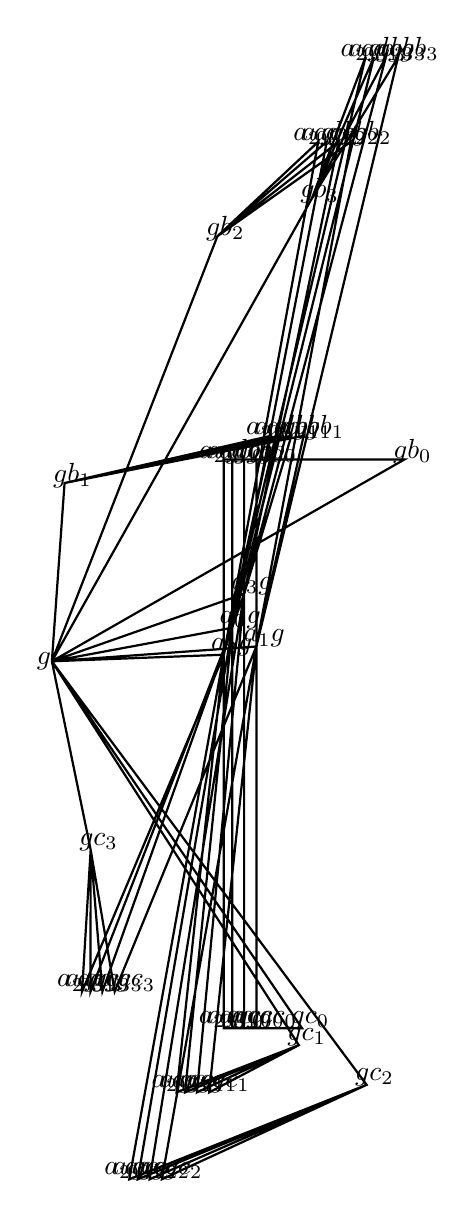
\begin{tikzpicture}
            \draw[thick](0,0)(0,0) -- (4.4786223903210995,2.5637912672429493) -- (2.290960484730933,2.5637912672429493) -- (2.290960484730933,0.4259199515847812) -- (0,0)
(0,0) -- (0.16122570022169713,2.264078505882993) -- (2.890960484730933,2.864078505882993) -- (2.290960484730933,0.4259199515847812) -- (0,0)
(0,0) -- (2.1024598685156057,5.398421037249038) -- (3.490960484730933,6.598421037249039) -- (2.290960484730933,0.4259199515847812) -- (0,0)
(0,0) -- (3.2999389034243185,5.873589167895953) -- (4.090960484730933,7.673589167895953) -- (2.290960484730933,0.4259199515847812) -- (0,0)
(0,0) -- (4.4786223903210995,2.5637912672429493) -- (2.597432367708243,2.5637912672429493) -- (2.597432367708243,0.188104617393947) -- (0,0)
(0,0) -- (0.16122570022169713,2.264078505882993) -- (3.197432367708243,2.864078505882993) -- (2.597432367708243,0.188104617393947) -- (0,0)
(0,0) -- (2.1024598685156057,5.398421037249038) -- (3.797432367708243,6.598421037249039) -- (2.597432367708243,0.188104617393947) -- (0,0)
(0,0) -- (3.2999389034243185,5.873589167895953) -- (4.397432367708243,7.673589167895953) -- (2.597432367708243,0.188104617393947) -- (0,0)
(0,0) -- (4.4786223903210995,2.5637912672429493) -- (2.18354959678122,2.5637912672429493) -- (2.18354959678122,0.08362839432419879) -- (0,0)
(0,0) -- (0.16122570022169713,2.264078505882993) -- (2.7835495967812203,2.864078505882993) -- (2.18354959678122,0.08362839432419879) -- (0,0)
(0,0) -- (2.1024598685156057,5.398421037249038) -- (3.3835495967812204,6.598421037249039) -- (2.18354959678122,0.08362839432419879) -- (0,0)
(0,0) -- (3.2999389034243185,5.873589167895953) -- (3.98354959678122,7.673589167895953) -- (2.18354959678122,0.08362839432419879) -- (0,0)
(0,0) -- (4.4786223903210995,2.5637912672429493) -- (2.4417924136018088,2.5637912672429493) -- (2.4417924136018088,0.8569820094818837) -- (0,0)
(0,0) -- (0.16122570022169713,2.264078505882993) -- (3.041792413601809,2.864078505882993) -- (2.4417924136018088,0.8569820094818837) -- (0,0)
(0,0) -- (2.1024598685156057,5.398421037249038) -- (3.6417924136018085,6.598421037249039) -- (2.4417924136018088,0.8569820094818837) -- (0,0)
(0,0) -- (3.2999389034243185,5.873589167895953) -- (4.241792413601809,7.673589167895953) -- (2.4417924136018088,0.8569820094818837) -- (0,0)
(0,0) -- (3.1778185201788753,-4.66028523056511) -- (2.290960484730933,-4.66028523056511) -- (2.290960484730933,0.4259199515847812) -- (0,0)
(0,0) -- (3.136274947973518,-4.875113228025686) -- (1.6909604847309327,-5.475113228025686) -- (2.290960484730933,0.4259199515847812) -- (0,0)
(0,0) -- (3.997415810572874,-5.378606422891057) -- (1.0909604847309329,-6.578606422891057) -- (2.290960484730933,0.4259199515847812) -- (0,0)
(0,0) -- (0.49273691985722456,-2.3931993075571008) -- (0.490960484730933,-4.193199307557101) -- (2.290960484730933,0.4259199515847812) -- (0,0)
(0,0) -- (3.1778185201788753,-4.66028523056511) -- (2.597432367708243,-4.66028523056511) -- (2.597432367708243,0.188104617393947) -- (0,0)
(0,0) -- (3.136274947973518,-4.875113228025686) -- (1.9974323677082428,-5.475113228025686) -- (2.597432367708243,0.188104617393947) -- (0,0)
(0,0) -- (3.997415810572874,-5.378606422891057) -- (1.397432367708243,-6.578606422891057) -- (2.597432367708243,0.188104617393947) -- (0,0)
(0,0) -- (0.49273691985722456,-2.3931993075571008) -- (0.7974323677082431,-4.193199307557101) -- (2.597432367708243,0.188104617393947) -- (0,0)
(0,0) -- (3.1778185201788753,-4.66028523056511) -- (2.18354959678122,-4.66028523056511) -- (2.18354959678122,0.08362839432419879) -- (0,0)
(0,0) -- (3.136274947973518,-4.875113228025686) -- (1.58354959678122,-5.475113228025686) -- (2.18354959678122,0.08362839432419879) -- (0,0)
(0,0) -- (3.997415810572874,-5.378606422891057) -- (0.9835495967812202,-6.578606422891057) -- (2.18354959678122,0.08362839432419879) -- (0,0)
(0,0) -- (0.49273691985722456,-2.3931993075571008) -- (0.38354959678122036,-4.193199307557101) -- (2.18354959678122,0.08362839432419879) -- (0,0)
(0,0) -- (3.1778185201788753,-4.66028523056511) -- (2.4417924136018088,-4.66028523056511) -- (2.4417924136018088,0.8569820094818837) -- (0,0)
(0,0) -- (3.136274947973518,-4.875113228025686) -- (1.8417924136018087,-5.475113228025686) -- (2.4417924136018088,0.8569820094818837) -- (0,0)
(0,0) -- (3.997415810572874,-5.378606422891057) -- (1.2417924136018088,-6.578606422891057) -- (2.4417924136018088,0.8569820094818837) -- (0,0)
(0,0) -- (0.49273691985722456,-2.3931993075571008) -- (0.6417924136018089,-4.193199307557101) -- (2.4417924136018088,0.8569820094818837) -- (0,0)
;
\node at (2.390960484730933,2.6637912672429493) {$ a_{ 0  } gb_{ 0 } $};
\node at (2.990960484730933,2.964078505882993) {$ a_{ 0  } gb_{ 1 } $};
\node at (3.590960484730933,6.698421037249038) {$ a_{ 0  } gb_{ 2 } $};
\node at (4.190960484730932,7.773589167895953) {$ a_{ 0  } gb_{ 3 } $};
\node at (2.697432367708243,2.6637912672429493) {$ a_{ 1  } gb_{ 0 } $};
\node at (3.297432367708243,2.964078505882993) {$ a_{ 1  } gb_{ 1 } $};
\node at (3.897432367708243,6.698421037249038) {$ a_{ 1  } gb_{ 2 } $};
\node at (4.497432367708242,7.773589167895953) {$ a_{ 1  } gb_{ 3 } $};
\node at (2.2835495967812203,2.6637912672429493) {$ a_{ 2  } gb_{ 0 } $};
\node at (2.8835495967812204,2.964078505882993) {$ a_{ 2  } gb_{ 1 } $};
\node at (3.4835495967812204,6.698421037249038) {$ a_{ 2  } gb_{ 2 } $};
\node at (4.08354959678122,7.773589167895953) {$ a_{ 2  } gb_{ 3 } $};
\node at (2.541792413601809,2.6637912672429493) {$ a_{ 3  } gb_{ 0 } $};
\node at (3.141792413601809,2.964078505882993) {$ a_{ 3  } gb_{ 1 } $};
\node at (3.7417924136018086,6.698421037249038) {$ a_{ 3  } gb_{ 2 } $};
\node at (4.341792413601809,7.773589167895953) {$ a_{ 3  } gb_{ 3 } $};
\node at (2.390960484730933,-4.5602852305651105) {$ a_{ 0  } gc_{ 0 } $};
\node at (1.7909604847309328,-5.375113228025686) {$ a_{ 0  } gc_{ 1 } $};
\node at (1.190960484730933,-6.478606422891057) {$ a_{ 0  } gc_{ 2 } $};
\node at (0.590960484730933,-4.093199307557101) {$ a_{ 0  } gc_{ 3 } $};
\node at (2.697432367708243,-4.5602852305651105) {$ a_{ 1  } gc_{ 0 } $};
\node at (2.097432367708243,-5.375113228025686) {$ a_{ 1  } gc_{ 1 } $};
\node at (1.497432367708243,-6.478606422891057) {$ a_{ 1  } gc_{ 2 } $};
\node at (0.8974323677082431,-4.093199307557101) {$ a_{ 1  } gc_{ 3 } $};
\node at (2.2835495967812203,-4.5602852305651105) {$ a_{ 2  } gc_{ 0 } $};
\node at (1.6835495967812202,-5.375113228025686) {$ a_{ 2  } gc_{ 1 } $};
\node at (1.0835495967812203,-6.478606422891057) {$ a_{ 2  } gc_{ 2 } $};
\node at (0.48354959678122034,-4.093199307557101) {$ a_{ 2  } gc_{ 3 } $};
\node at (2.541792413601809,-4.5602852305651105) {$ a_{ 3  } gc_{ 0 } $};
\node at (1.9417924136018088,-5.375113228025686) {$ a_{ 3  } gc_{ 1 } $};
\node at (1.341792413601809,-6.478606422891057) {$ a_{ 3  } gc_{ 2 } $};
\node at (0.7417924136018089,-4.093199307557101) {$ a_{ 3  } gc_{ 3 } $};
\node at (-0.1,0) {$ g $};
\node at (2.390960484730933,0.5259199515847812) {$ a_{ 0 }g $};
\node at (2.697432367708243,0.288104617393947) {$ a_{ 1 }g $};
\node at (2.2835495967812203,0.1836283943241988) {$ a_{ 2 }g $};
\node at (2.541792413601809,0.9569820094818837) {$ a_{ 3 }g $};
\node at (4.578622390321099,2.6637912672429493) {$ gb_{ 0 } $};
\node at (0.2612257002216971,2.364078505882993) {$ gb_{ 1 } $};
\node at (2.202459868515606,5.498421037249038) {$ gb_{ 2 } $};
\node at (3.3999389034243186,5.973589167895953) {$ gb_{ 3 } $};
\node at (3.2778185201788754,-4.5602852305651105) {$ gc_{ 0 } $};
\node at (3.2362749479735182,-4.7751132280256865) {$ gc_{ 1 } $};
\node at (4.0974158105728735,-5.278606422891057) {$ gc_{ 2 } $};
\node at (0.5927369198572245,-2.2931993075571007) {$ gc_{ 3 } $};

            \end{tikzpicture}
            \end{center}
            \caption{Square of the complex, with edges $(g,ag), (agb, gb) \in E_A,
            (g,gb), (agb, ag) \in E_B.$ \label{fig:square}
            }
            \end{figure}
 
%\end{multicols*}
  % \printbibliography 
\end{document}

 